%use in documents with \subfile{tex/intro}
\documentclass[../../master.tex]{subfiles}

\begin{document}

\subsection{Preliminary Experimental Results}
\label{sub:exp_results}

To test the designed sequences, an assay based on the self-splicing mechanism of the \textit{Azoarcus} group I intron (see \autoref{sub:theory:azoarcus_selfsplicing}) was developed by the partner group in Paris, France.
Currently, preliminary results are available only for a selection of designed sequences of the \texttt{proto} set.
These sequences had to be post-processed to fit experimental requirements, i.e. they had to be truncated, and the first three 5'-nucleotides were replaced with the native IGS, and the 3'-terminal nucleotide was set to \texttt{G}.

The results of a negative control experiment with known non-catalytically active RNAs are not yet available.
Therefore, the following paragraphs do not represent the latest experimental results.

\subsubsection{Mechanism of the Self-Splicing Assay}
\label{ssub:exp_results:assay}

The goal of the assay was to screen a small pool of designed synthetic introns for self-splicing and ligating activity at their 3' end.

Therefore, a synthetic 3'-exon was appended to the potential synthetic catalysts.
A short RNA substrate with the trinucleotide \texttt{CAU} at its 3' end was added to bind to the introns IGS.
This setup corresponds to the \emph{pre-2S} state of the self-splicing mechanism in the native intron (see \autoref{fig:selfsplicing}).
Catalytically active synthetic introns were expected to be able to splice the synthetic exon and ligate it to the substrate by the same mechanism.

A second RNA substrate with a 5'-oligonucleotide \texttt{GGCAU} containing the IGS recognition motif was used for the reverse reaction.
Since the 3'-terminal nucleotide of the synthetic introns was \texttt{G}, this nucleotide would be expected to bind to the guanosine binding site and splice the substrate from its 5'-oligonucleotide, followed by ligation of the substrate to the 3' end in catalytically active introns (\emph{post-2S} in \autoref{fig:selfsplicing}).

In total, three different states were expected for catalysts; the intron with the synthetic 3'-exon, the intron without any exons attached, and the intron with the second substrate substituting the 3'-exon.
However, the presence of the third state would be sufficient to indicate the success of the assay.

\subsubsection{Assay Results}
\label{ssub:exp_results:assayresults}

%\todo{not sure if I should include the details of incubation, PCR, etc.}

Template DNA of the designed sequences with a synthetic exon added to the 3' end and a promoter sequence was ordered, amplified and purified by polymerase chain reaction (PCR) and transcribed into RNA by the partner group in Paris.

The designed RNA sequences were incubated in small pools of multiple sequences with the two substrates added to conduct the assay.
Afterwards, a reverse transcription (RT-PCR) was initiated with a primer complementary to the 3' end of the second substrate.
That way, only introns with this substrate would be reversely transcribed into DNA.
So far, except for a control run using the native \textit{Azoarcus} intron, no activity was detected.
Therefore, the reversely transcribed DNA was amplified to increase a potential signal.
After the amplification, bands corresponding to sequences roughly \unit[200]{nt} long were observed for the designed synthetic introns as well as the native
intron (\autoref{fig:gel_proto}).

\begin{figure}[!ht]
	\centering
	\begin{tikzpicture}
		\node[anchor=south west] (image) at (0,0) {
			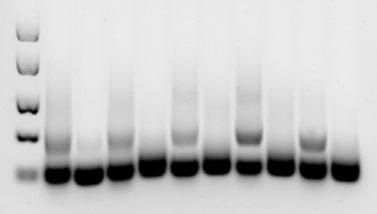
\includegraphics[width=0.7\textwidth]{pic/results/designs/gel_proto_cropped.png}
		};
		\node (sample) at (9.25,5.5) {\texttt{proto}};
		\node (brace) at (9.25,5.0) {$\overbrace{\hphantom{spaaaace}}$};
		\node (azo) at (3.1,5.5) {\textit{Azoarcus}};
		\node (brace1) at (3.1,5.0) {$\overbrace{\hphantom{spaaaaaaaaaaace}}$};
		\node[anchor=east] (50nt) at (0.7,1.25) {\unit[50]{nt}};
		\node[anchor=east] (200nt) at (0.7,2.35) {\unit[200]{nt}};
		\draw (1.35, 4.8) -- (1.35, 0.8);
		\draw (3.1, 4.8) -- (3.1, 0.8);
		\draw (4.85, 4.8) -- (4.85, 0.8);
		\draw (6.65, 4.8) -- (6.65, 0.8);
		\draw (8.4, 4.8) -- (8.4, 0.8);
		
		
	\end{tikzpicture}
	\caption[Gel of a Splicing Assay]{Gel obtained by gel-electrophoresis of reversely transcribed and amplified DNA from the assayed introns.
		Vertical lines separate pools of different design methods. 
		Unlabelled pools originate from methods not part of this thesis.
		Lanes labelled \textit{Azoarcus} contain DNA corresponding to the native intron as a control.
		The right lane of each pool was obtained from assay runs without any substrate added.
		Camille Lambert generously provided the gel (Laboratoire de Biochimie, ESPCI Paris, France).
	}\label{fig:gel_proto}
\end{figure}

Due to the selective RT-PCR, this band should correspond to catalytically active synthetic introns from at least one of the designed sequences in the pool.

The dominant bands at around \unit[50]{nt} correspond to non-specific DNA since the RT-PCR was highly sensitive.
These bands were also visible in control runs without any substrate added.

\end{document}
